%!TEX root = ../dissertation.tex


\chapter{Discussion}
\label{discussion}


The motivation for this research was driven by the experiences with high resolution numerical models in the NOAA Hazardous Weather Testbed, in particular the NSSL-WRF, along with the needs of the ``Warn-on-Forecast'' (WoF) initiative.
One aim of the WoF initiative is to transform the warning paradigm of rare convective events from one where RCE warnings are based almost entirely on observations to one where RCE warnings are based on short-term, high resolution numerical forecasts of an RCE occurring.
A key challenge for the WoF paradigm is to produce probabilistic guidance for the occurrence of RCEs that has a high degree of statistical reliability and resolution and is unambiguous for users to interpret.


This is especially challenging since these phenomena will not be explicitly resolved in larger domain model configurations for many years to come (e.g., explicit prediction of tornadoes will require grid spacing on the order of a few tens of meters).
One possibility for overcoming this problem is to identify ``extreme'' model-generated features that have strong correlations with observed severe convective phenomena, and then use the former as surrogates for the severe phenomena in question.
This ``surrogate-severe'' (SS) approach is fundamentally different from traditional applications of numerical weather prediction for severe weather because it is phenomenon based.
In particular, it relies on identification of explicit convective phenomena rather than environmental conditions that might support such phenomena.


\cite{Sobash2011} established the viability of this approach using several different SS diagnostic quantities.
Among the quantities they examined, model-generated updraft helicity (UH) appeared to show the strongest correlation with observed reports of severe weather.
[UH is a measure of mid-level rotation in model-predicted updrafts and subjective assessments suggest that it is a useful surrogate for supercell thunderstorms \citep{Kain2010}, even when these storms are only crudely represented on the WRF model's native grid \citep{Kain2008}.]
Subjective assessments in the HWT convinced participants that SS quantities from high resolution models had the potential to offer guidance to forecasters as to the vicinity (in time and space) of RCE occurrence, but not necessarily the exact location.


The fact that subjective assessments of high resolution numerical model forecasts suggest that forecasts of RCEs are in the vicinity of observations of RCEs, but are not necessarily collocated, highlights the need for the forecast to be expressed probabilistically.
One way to do this is to utilize an ensemble of high resolution numerical models to quantify the spatial uncertainty in the location of the forecast RCEs.
Unfortunately, the infrequent nature of rare events makes it unlikely that two separate high-resolution model forecasts would place extreme model-generated convective storm phenomena at the same grid point, even for generally similar mesoscale forecasts.
Thus, ensemble generated probabilities of RCE occurrence at a given grid point are typically extremely small.
This is consistent with the limited predictability on the convective scale and the associated low climatological frequency of rare events, which makes it difficult to convey statistically meaningful severe weather threats to the user community \citep{Murphy1991}.


Informal conversations with operational meteorologists in the HWT suggest that both forecasters and users of hazardous weather information may not respond appropriately to the very small probability values that result from creating ensemble probabilities of RCE occurrence on a fine grid, as is the cause with storm scale ensemble forecast systems.
One potential remedy to this problem was offered by \cite{Sobash2011}.
Instead of using an ensemble to generate a probabilistic forecast, their method utilized a a single deterministic forecast and applied a ``neighborhood''-based approach that is rooted in the concepts of \cite{Theis2005} and \cite{Brooks1998}.
This neighborhood approach consists of two steps.
The first step consists of taking binary grid point forecasts of occurrence of specific events and expanding their spatial extent by converting all grid points within a specified ``neighborhood'' into forecasts of occurrence for the given event.
For example, consider a case in which a single grid point from a high resolution numerical model with grid spacing of \mbox{4 km} grid is forecast to have a phenomenon occur.
Furthermore consider that a neighborhood of \mbox{40 km} is specified
The first step of the neighborhood approach takes all grid points within the specified neighborhood of the forecast grid point, \mbox{40 km} radius in this example, and converts those grid points into forecasts of the phenomenon's occurrence.
This effectively increases the area for which the phenomenon is forecast.


The second step involves using kernel density estimation to convert the neighborhood forecasts into forecasts of probability of occurrence.
\cite{Sobash2011} employed a two-dimensional isotropic Gaussian kernel in their study, but had no method of optimally selecting the appropriate bandwidth.
Their solution was to evaluate multiple choices of bandwidth and select the one that verified the best.


One negative to the neighborhood approach put forth by \cite{Sobash2011} is that by using a neighborhood, the specificity offered by high-resolution numerical models is diminished.
No longer is a forecaster examining the probability of a phenomenon occurring on a given grid point, instead the forecaster is examining the probability of a phenomenon occurring within the defined neighborhood.
However, given the limited predictability on the convective grid scale and the comparatively low probability values at the grid point, use of a neighborhood is typically considered an acceptable method to identify a region of enhanced threat.


The method put forth by \cite{Sobash2011} relies on accurate observations of the phenomenon being predicted to assess the quality of the resulting probabilistic forecasts.
This poses significant limitations due to the lack of quality observations of these phenomena.
As previously noted, numerical guidance of severe thunderstorms has improved in recent years with the advent of convection-allowing models and high temporal resolution storm-attribute parameters (e.g., updraft-helicity, downdraft intensity, graupel loading, etc; \citealp{Kain2010}).
Unfortunately, however, corresponding observational datasets with spatial and temporal coherence comparable to the model data are not available.


Quantitative precipitation forecasts, on the other hand, pose challenges to operational forecasters similar to those posed by severe thunderstorm forecasts.
One important difference is that quantitative precipitation forecasts have comparatively robust verification datasets.
Thus, one approach to improving the quality of numerical models' probabilistic forecasts of RCEs is to develop and refine techniques of predicting and calibrating extreme precipitation ``events''.
After these enhancements have been fully evaluated using extreme precipitation events the refined methods can be applied to the original severe thunderstorm prediction problem.


This study did just that.
It is a proof-of-concept for using numerical forecasts of explicit phenomenon-based RCE to create objectively calibrated probabilistic forecasts.
This proof-of-concept builds on the twork of \cite{Sobash2011} achieved by using grid point forecasts of heavy precipitation events (defined to be either \mbox{12.7 mm} or \mbox{25.4 mm} in \mbox{6 hr}) and the corresponding verification datasets, to build on the work of \cite{Sobash2011}.
Furthermore, it does without the use of a neighborhood, allowing forecasters to utilize the higher specificity offered by high resolution numerical models as compared to coarser resolution models, such as the NAM.
The objectively calibrated probabilistic forecasts are achieved by first computing a two-dimensional frequency distribution of observed precipitation event locations relative to forecasts of precipitation events.
Then, these two-dimensional composites are used to determine the necessary parameters of an analytical function that can be used in the kernel density estimation step of \cite{Sobash2011}.
Assessing the utility of such an approach with two very different high resolution datasets --- 1) 48-months of high resolution output from the real-time NSSL-WRF model; and 2) the individual member forecasts for the 119 time periods from the 2010 and 2011 CAPS SSEF --- generally indicates this technique has the potential to produce skillful probabilistic forecasts derived from a single numerical forecast.


NSSL-WRF probabilistic forecasts of precipitation exceeding \mbox{25.4 mm} in \mbox{6 hr}, utilizing the approach put forth in this study, were subjectively evaluated during the 2011 NOAA HWT SFE.
During this subjective assessment operational forecasters expressed concern about the resulting probability field, particularly the smooth appearance and low amplitude.
Although a valid concern, the character of the probability fields is inherently linked to the underlying numerical model's ability to accurately predict the exact location of ``events''.
When a model's two-dimensional histogram has a large area of relatively uniform observed event occurrence, indicative of relatively large model spatial uncertainty, the fitted analytic function generates broad, low-amplitude probabilities.
Conversely, when the higher observed event occurrence in the two-dimensional histogram is more concentrated, indicating a reduction in model spatial uncertainty, the analytic function produces sharper, higher-amplitude probabilities.
Simply stated, this technique objectively quantifies the spatial uncertainty associated with the deterministic forecasting skill of the modeling system.
Thus, concerns about overly smooth, low-amplitude probability fields are directly related to the deterministic model's ability to accurately predict the location of the forecast events.


Some mitigation of the aforementioned concerns are possible without a complete overhaul of the modeling system.
Evaluations suggest that forecast lead time, geographic location, as well as meteorological season and regime all impact the two-dimensional frequency histogram of observations relative to forecasts.
This is particularly evident in the variability in the two-dimensional frequency histograms from the individual members of the CAPS SSEF, which were limited to 59 time periods and a single meteorological season.
Thus, instead of creating a single analytic function to handle all scenarios, as was done in this study, one might create a continuum of analytic functions dependent on factors such as forecast lead time, meteorological regime, and season of the year.
Preliminary examination suggests that all of these sensitivities are operative, but quantifying them will be challenging and will serve as the basis for future investigations.


One additional source of error that has not been mentioned until now is the forecast bias of each numerical forecast model.
As the forecast bias increases, the resulting probability forecasts change because of: 1) the number of forecast grid points increases; and 2) changes to the two-dimensional composites alter the fitting parameters.
In the case of the NSSL-WRF evaluations, the forecast bias was largely negligible over the forecast dataset.
This is because the forecast bias for the NSSL-WRF forecast periods was nearly one (Figures \ref{single_25quant}, \ref{single_12quant}, and \ref{nssl-wrf_bias}).
Unfortunately, the forecast bias was not always near unity for the members of the CAPS SSEF (e.g. \mbox{Figures \ref{s4cn_arw_ecdf_12mm_400km} and \ref{s4cn_nmm_ecdf_12mm_400km}}).


One approach to bias correcting the forecasts is to utilize quantile replacement.
This is achieved by computing the empirical cumulative distribution function for both the observations and the forecasts for the training period.
Then the quantile of the desired threshold is found from the empirical cumulative distribution of the observations.
Next this ``observed quantile'' is used to find the forecast threshold that corresponds to the same quantile from the empirical cumulative distribution of the forecast.
This assures that the same fraction of forecasts occurring above the threshold and below the threshold is equal to the fraction of observations occurring above the threshold to the observations occurring below the threshold.


Unfortunately, this approach only improves the resulting forecasts if the empirical cumulative distribution function for the forecast data is statistically similar to the empirical cumulative distribution function for the training data.
If this is not the case, the resulting probability forecasts could end up being worse as a result of the forecast bias being worse for the forecast data than for the training data.
The quantile replacement approach to bias correction was used to try and improve the forecasts from both the NSSL-WRF and the CAPS SSEF.
In both cases, the bias corrected forecasts offered little, if any, improvement to the reliability --- and in the case of the NSSL-WRF made the forecasts less reliable.
This is due to the fact the empirical cumulative distribution function for the training data was statistically different than for the forecast data.
For example, the forecast bias for the CAPS SSEF members was highly dependent on the specific time periods chosen for the training and forecast periods.
This is attributed to the occurrence of a handful of high amplitude precipitation time periods.
Depending on the exact number of these high amplitude time periods in each of the training or forecast dataset, the resulting empirical cumulative distribution functions were one of several distributions (\mbox{Figure \ref{s4cn_arw_ecdf_12mm_400km} and \ref{s4cn_nmm_ecdf_12mm_400km}}) making this form of bias-correction untractable.


Lastly, it is important to discuss the role of ensemble prediction systems in producing probabilistic forecasts.
In this study, probabilistic forecasts from an ensemble prediction systems were limited to probabilistic forecasts from individual members.
A single ``ensemble probability'' was produced by taking the average of all the probabilistic forecasts from the ensemble's individual members.
As discussed in \mbox{Section \ref{ediscussion}}, the reliability of this single probabilistic forecast from the ensemble improved upon the individual members at the \mbox{25.4 mm} in \mbox{6 hr} threshold and was worse than the individual members at the \mbox{12.7 mm} in \mbox{6 hr} threshold.
Furthermore, it was shown that it is possible to produce probabilistic forecasts from each individual member that were more reliable than a probabilistic forecast generated by post-processing the ensemble forecast.
In light of this result, the question must be asked, ``What then is the role of the ensemble?''


Traditionally, ensemble prediction systems have been used to create probabilistic forecasts.
This is because well crafted ensemble prediction systems are likely to be more effective at sampling the range and character of possible solutions.
As previously mentioned, KDE-based approaches rely on the underlying numerical forecast to predict the occurrence of the phenomenon being forecast.
If the underlying numerical model does not forecast a phenomenon, KDE-based statistical post-processing will not produce any forecast probabilities of that phenomenon.
This is where an ensemble prediction system can add benefit to KDE-based statistical post-processing --- by providing additional realizations from which a KDE-based statistical post-processing technique can be used.


Taking a step back, the KDE-based post-processing technique proposed in this work has the potential to produce probabilistic forecasts from each member that are near perfect reliability (e.g., the SSEF forecasts at the \mbox{12.7 mm} in \mbox{6 hr} threshold used in this study).
It is not readily apparent what to do with a set of fifteen probabilistic forecasts that differ between one another but are statically reliable.
Each probabilistic forecast is statistically correct, but varies between one another.
One possible solution here is to utilize both the deterministic aspect of the individual SSEF members, along with their corresponding probabilistic aspect.
For example forecasters can examine the evolution of the forecast in deterministic space, and see the resulting spatial uncertainty of that model.











%%% FIGURES %%%

\clearpage
\begin{figure}[cc]
    \centering
    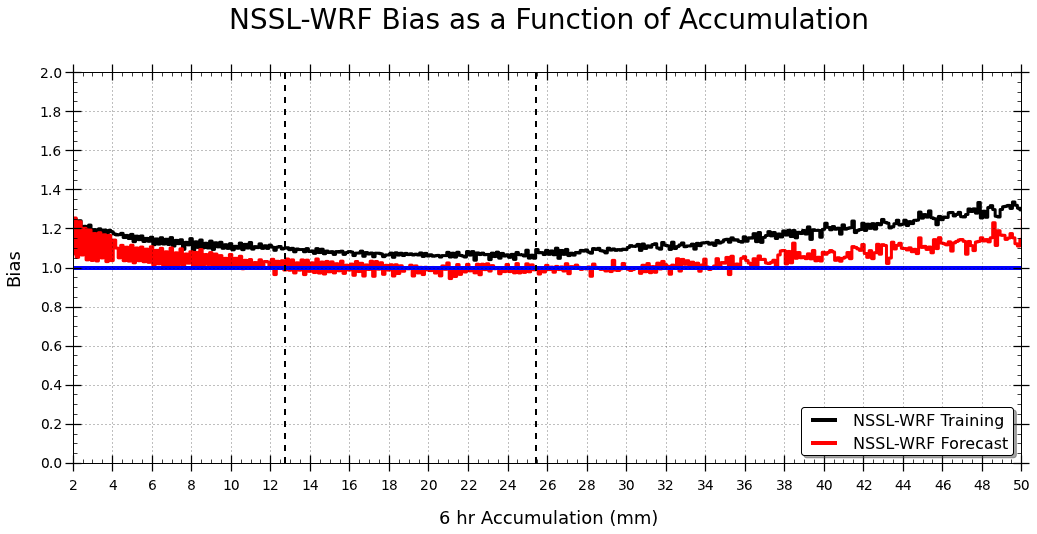
\includegraphics[width=\textwidth, height=\textheight, keepaspectratio]{%
    ./discussion/figs/nssl-wrf_bias}\\
    \caption{}
    \label{nssl-wrf_bias}
\end{figure}


\clearpage
\begin{figure}[cc]
    \centering
    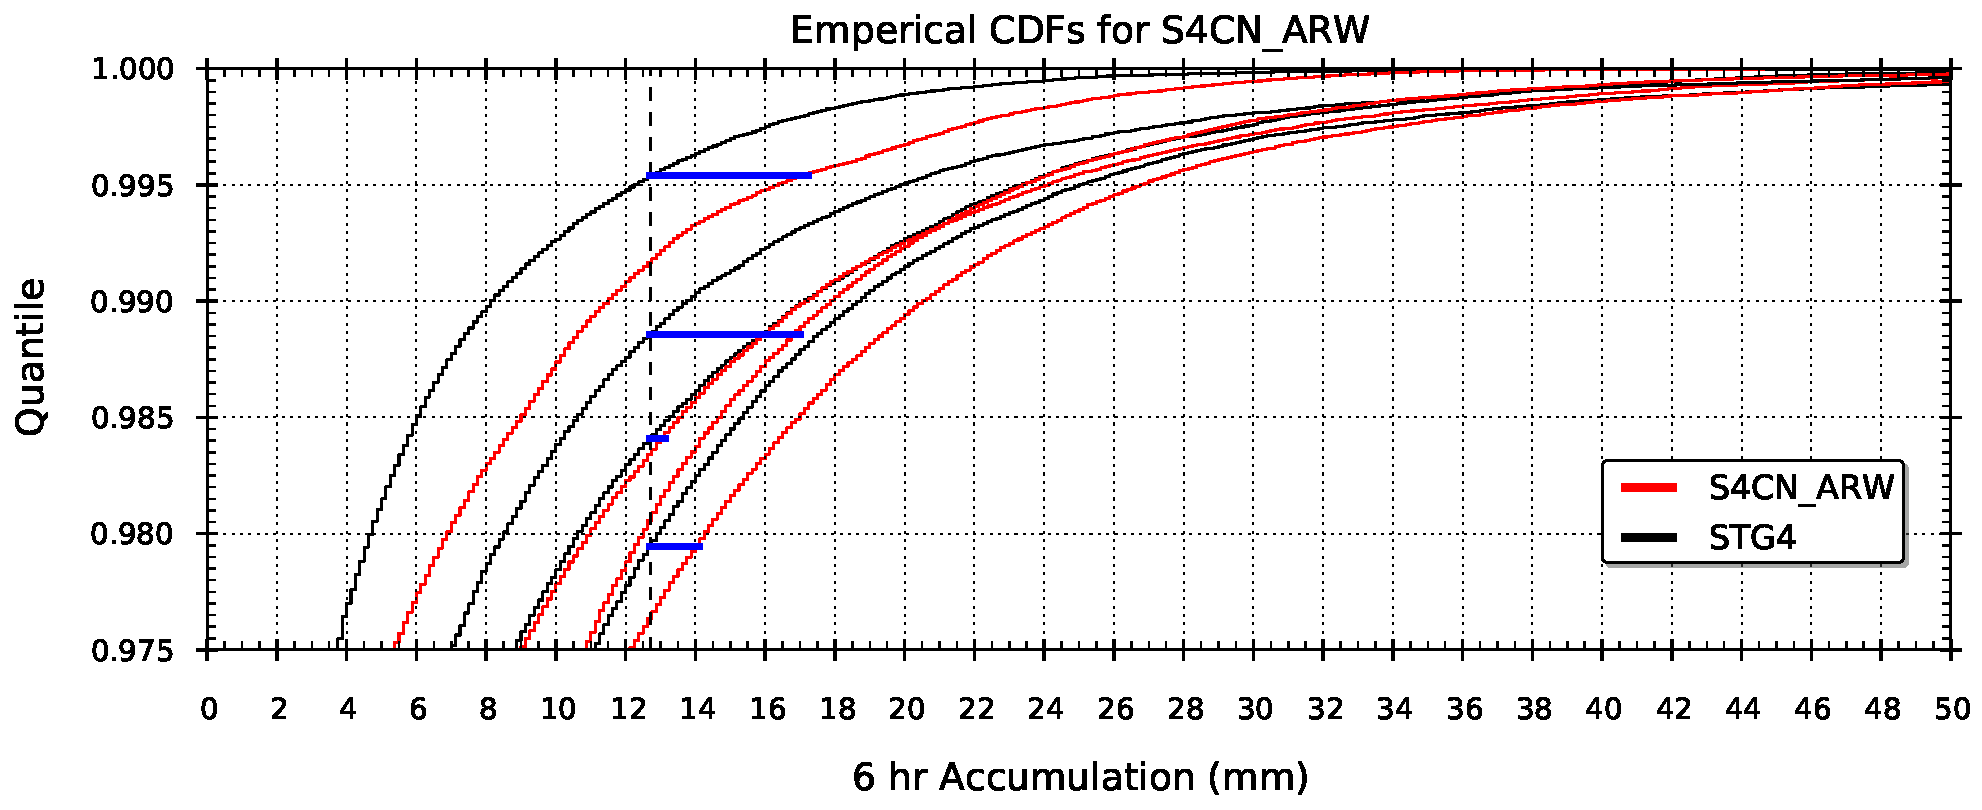
\includegraphics[width=\textwidth, height=\textheight, keepaspectratio]{%
    ./discussion/figs/ecdf_12mm_400km_s4cn_arw.pdf}\\
    \caption{}
    \label{s4cn_arw_ecdf_12mm_400km}
\end{figure}


\begin{figure}[cc]
    \centering
    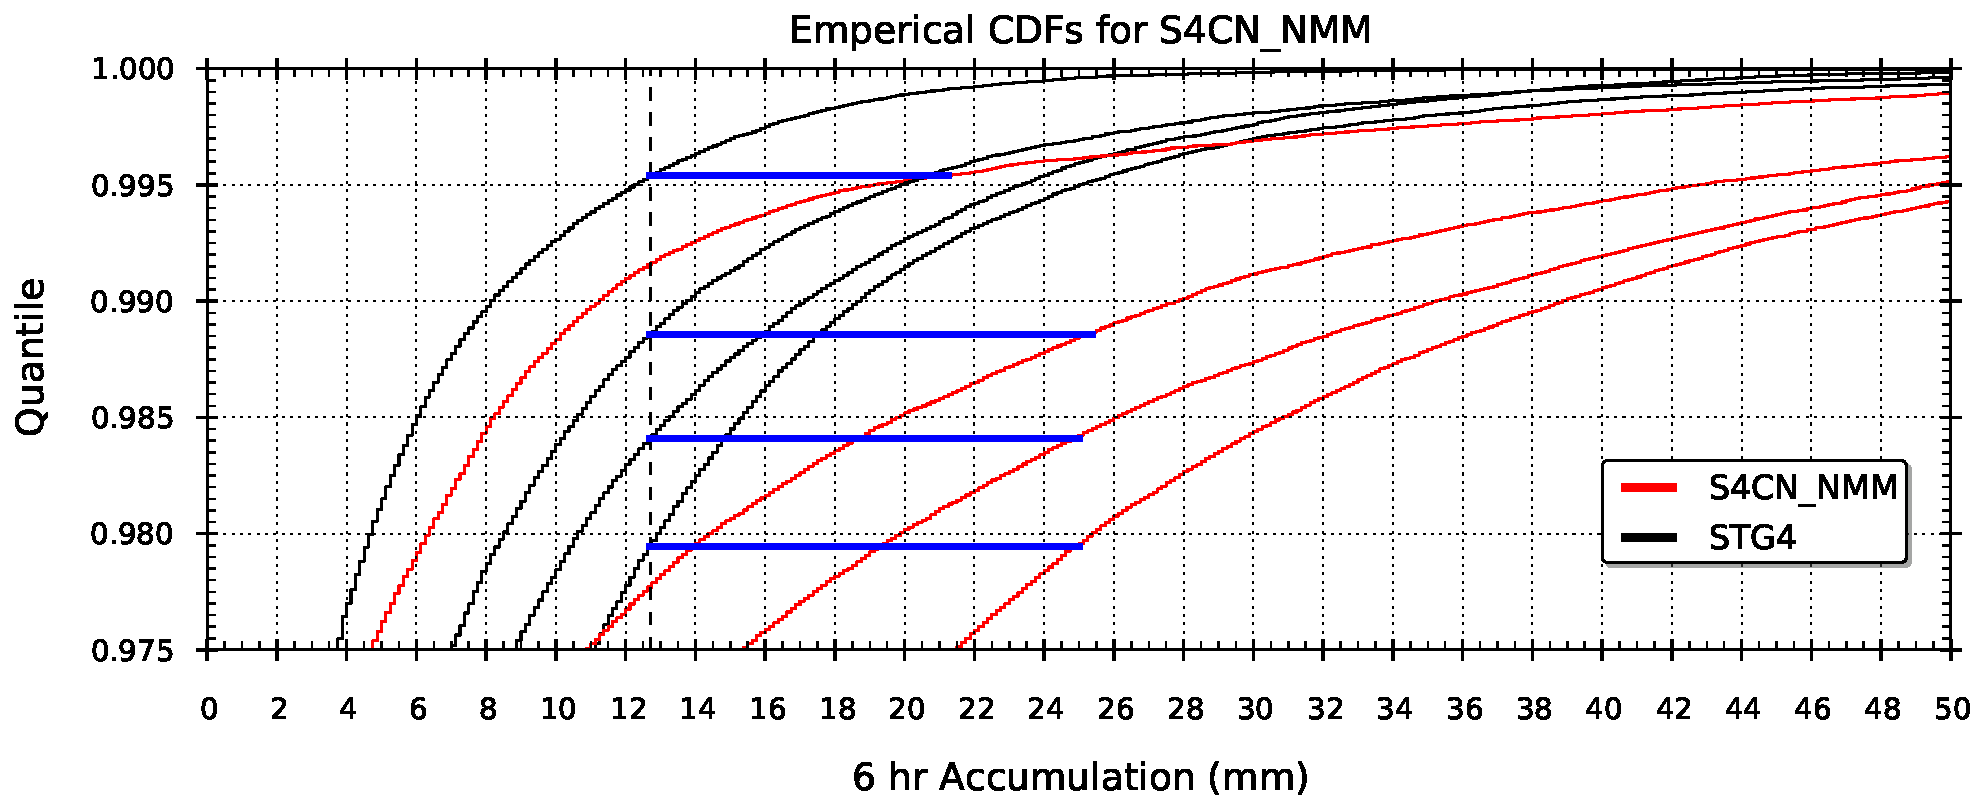
\includegraphics[width=\textwidth, height=\textheight, keepaspectratio]{%
    ./discussion/figs/ecdf_12mm_400km_s4cn_nmm.pdf}\\
    \caption{}
    \label{s4cn_nmm_ecdf_12mm_400km}
\end{figure}
